\documentclass{article}
\usepackage{graphicx}
\usepackage{listings}
\usepackage{xcolor}
\usepackage{hyperref}
\usepackage{geometry}
\geometry{a4paper, margin=1in}
\title{Grafici dell'utilizzo di memoria heap da parte degli algoritmi di ricerca}
\author{Adriano Oliviero}
\date{	oday}
\begin{document}
\maketitle
\tableofcontents
\newpage
\section{Grafici e Risultati}
Di seguito sono riportati alcuni grafici che visualizzano i risultati sperimentali degli algoritmi di ricerca applicati ai dataset:
\subsection{Dataset: email-Enron.txt.gz}
\subsubsection{Algoritmo di ricerca: bi-directional}
\begin{figure}[h]\centering
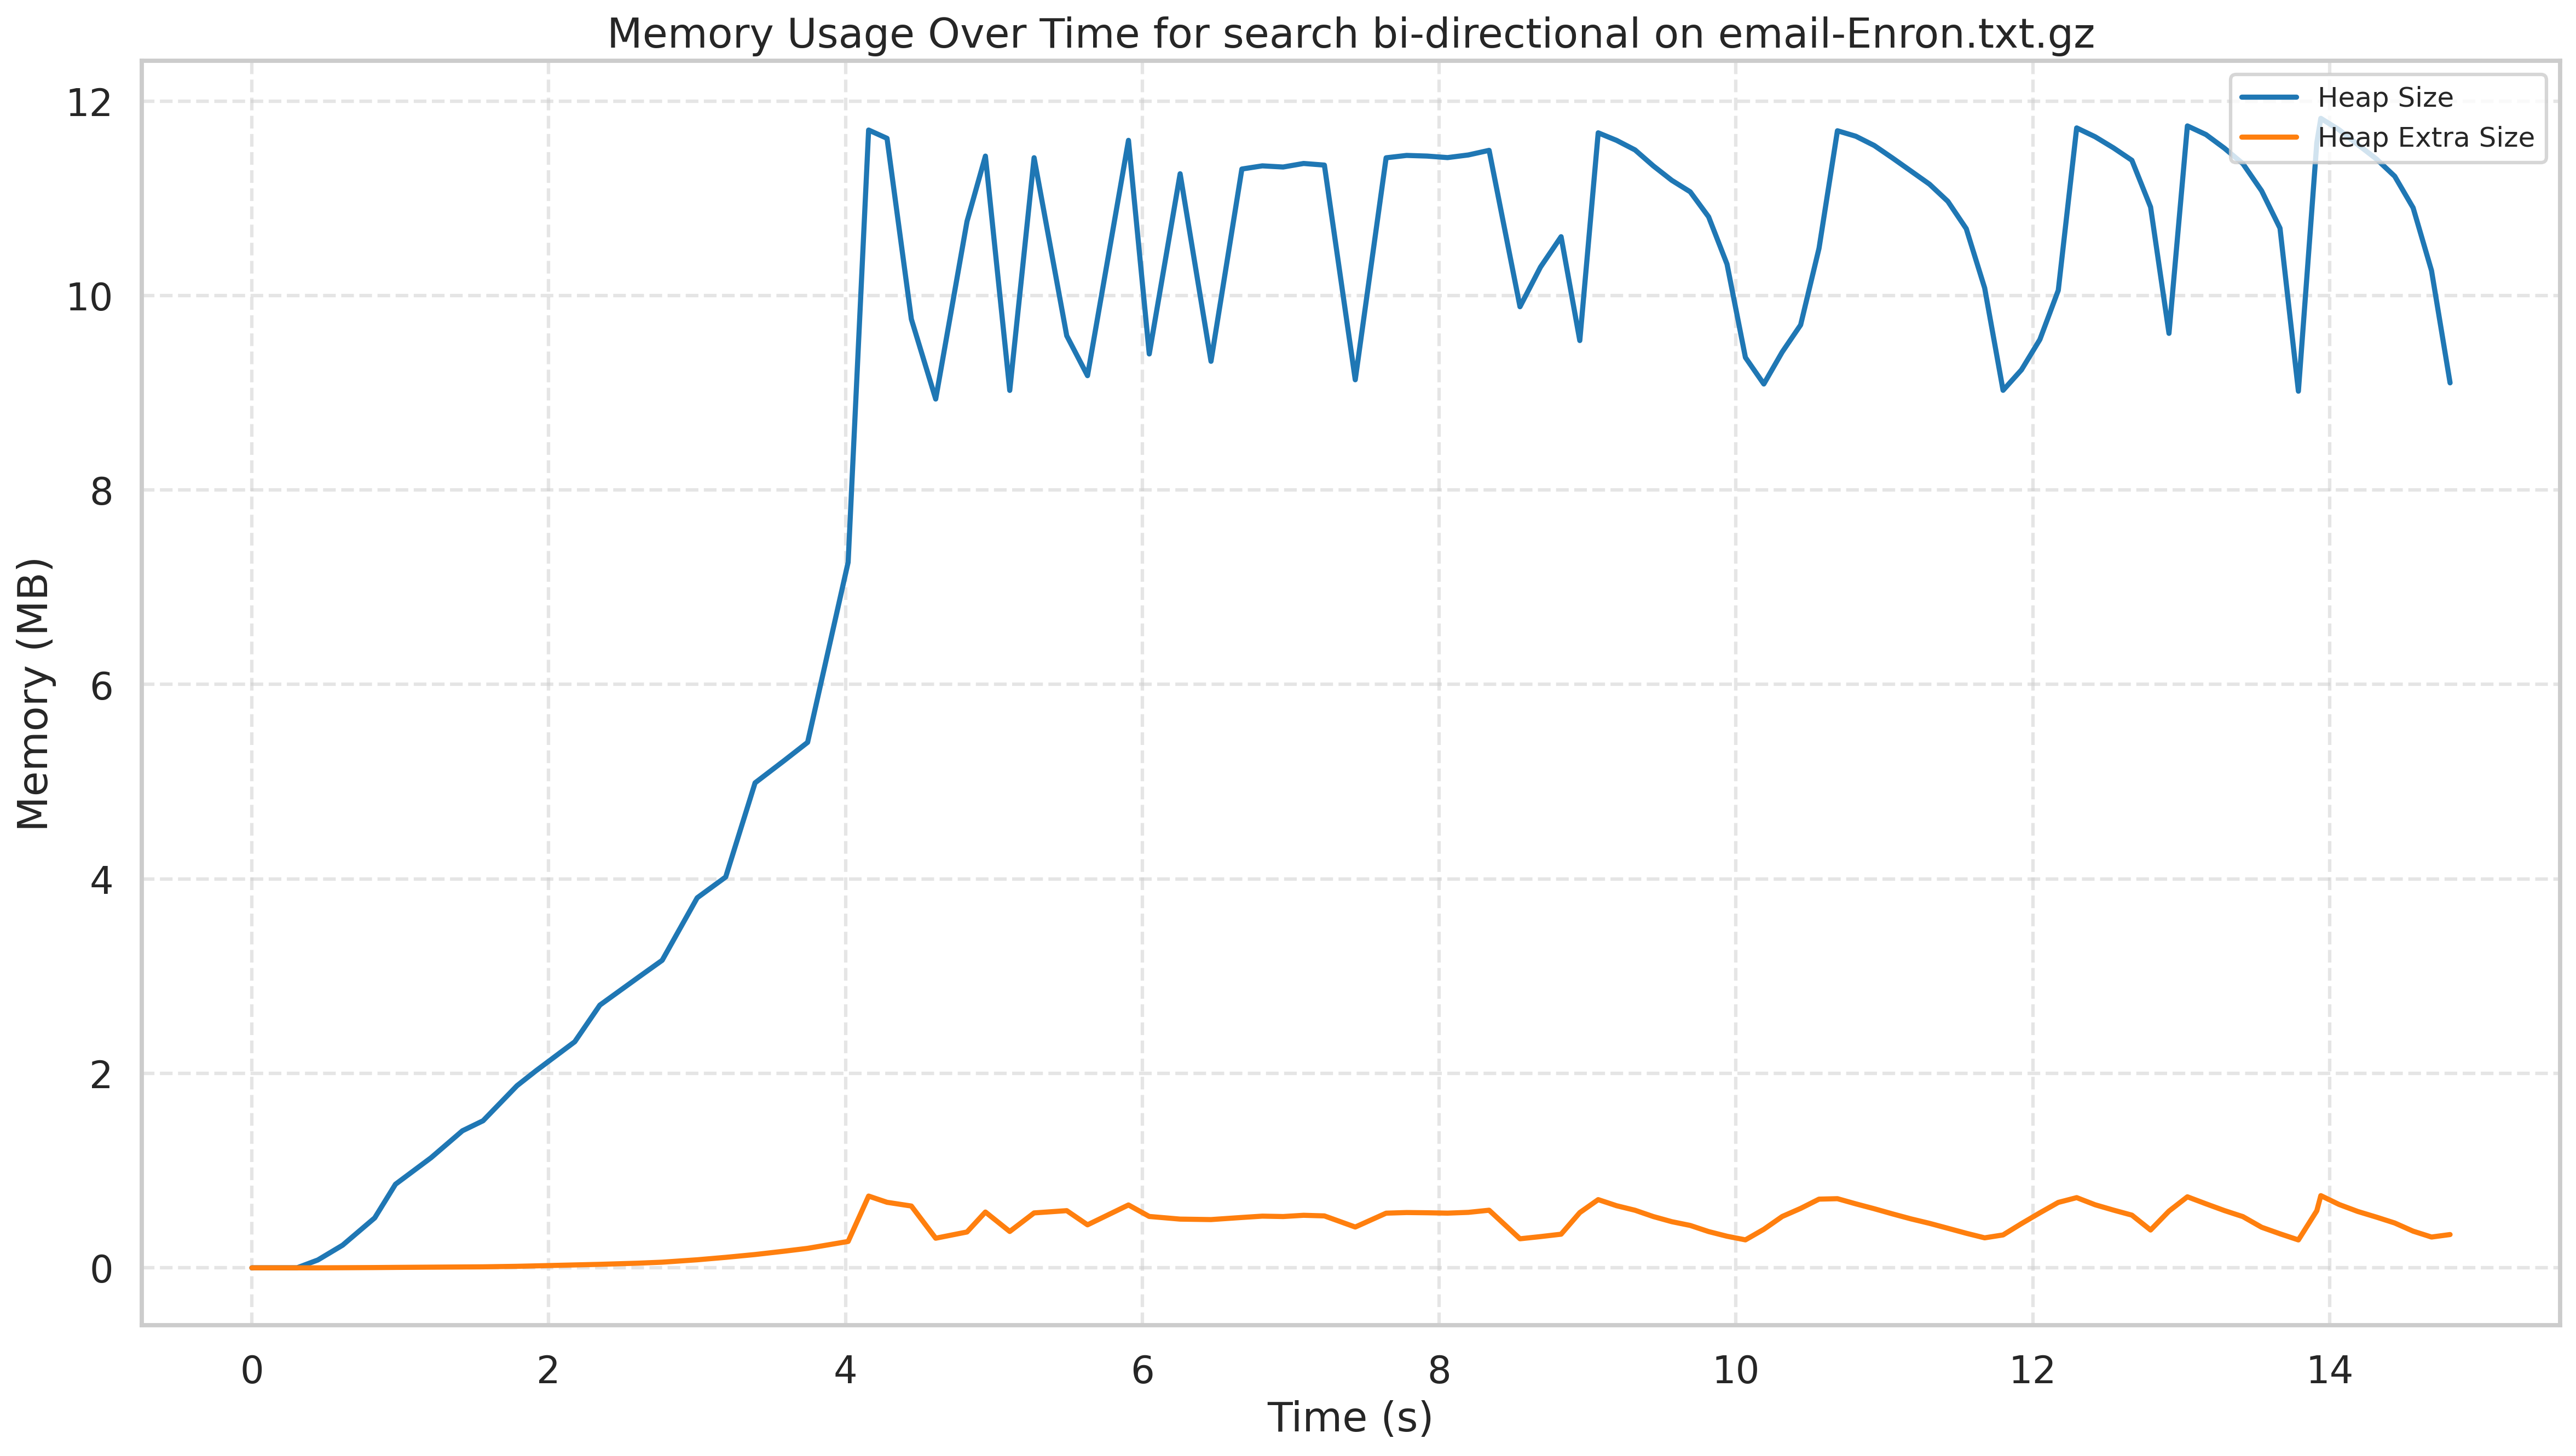
\includegraphics[width=\textwidth]{../plots/email-Enron_bi-directional.png}
\caption{Grafico: breadth-first su com-lj.ungraph}
\end{figure}
\end{document}